\documentclass[tikz,border=3pt]{standalone}
\usepackage[utf8]{inputenc}
\usepackage[T1]{fontenc}
\usepackage{libertinus}
\usepackage{amsmath,amssymb}
\usetikzlibrary{arrows.meta,calc,patterns,decorations.pathmorphing,decorations.markings,decorations.pathreplacing,bending}
\definecolor{UGblue}{RGB}{0,51,102}
\newcommand{\dbar}{\mathchar'26\mkern-12mu d}
\tikzset{
  >=Stealth,
  every node/.style={font=\small},
  caja/.style={draw,line width=0.9pt},
  pared/.style={draw,line width=1.6pt},
  ejes/.style={->,line width=0.8pt},
  adia/.style={draw,pattern=north east lines,pattern color=black!70,line width=0.5pt},
  gas/.style={fill=UGblue!8},
  punto/.style={fill,circle,inner sep=1.3pt},
  onda/.style={decorate,decoration={snake,amplitude=1.1pt,segment length=5pt,post length=3pt,pre length=0pt}},
}
\begin{document}
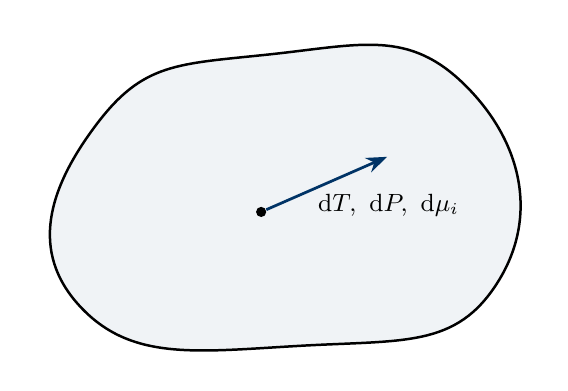
\begin{tikzpicture}
  \draw[smooth cycle,tension=0.9,fill=UGblue!6,line width=0.9pt] plot coordinates {(0,0.2) (2.8,-0.3) (5.3,0.5) (4.9,3.0) (2.4,3.4) (0.2,2.5)};
  \node[punto] (p) at (2.3,1.4) {};
  \draw[->,line width=1pt,UGblue] (p) -- (3.9,2.1);
  \node[below right] at (2.9,1.75) {$\mathrm{d}T,\ \mathrm{d}P,\ \mathrm{d}\mu_i$};
\end{tikzpicture}
\end{document}
